\chapter{Problem Formulation}
\label{ch:method}

Milestone~2 formulated the problem in two layers, a static layer (fixed spacecraft) and an
orbital layer (spacecraft on Keplerian orbits). This milestone optimises the orbital layer only,
with three changes agreed by the team: the mission duration $T$ becomes a decision variable
instead of a constant, the number of spacecraft $N$ is decided by the optimiser, and every orbit
is circular. This chapter gives the final formulation that both the \ac{SA} algorithm of
Chapter~\ref{ch:sa} and the \ac{GA} of Chapter~\ref{ch:ga} solve. The simulation that turns a design into the quantities used here is
described in Chapter~\ref{ch:orbital}.

\section{Problem statement}
A fleet of up to $N_{\max}$ identical spacecraft is sent to an irregular, rotating asteroid.
Every spacecraft flies its own circular orbit and carries the same narrow-angle camera. The
task is to decide \emph{how many} spacecraft to send, \emph{which orbit} each one flies and
\emph{how long} the mission lasts, so that together the spacecraft photograph as much of the
sunlit surface as possible with a usable image resolution, while sending as few spacecraft as
possible, using as little energy as possible and finishing as early as possible. The orbits
must stay at a safe distance from the asteroid and from each other, and no battery may run
down.

The problem is \emph{cooperative}: a surface facet that one spacecraft has already
photographed adds nothing to the coverage when another spacecraft photographs it again, so
the value of a spacecraft depends on what the rest of the fleet sees. The method only needs a
triangle mesh of the body, its gravitational parameter and its spin; it is applied to two real
asteroids, 433~Eros and 216~Kleopatra (Figure~\ref{fig:bodies}).

\begin{figure}[htbp]
\centering
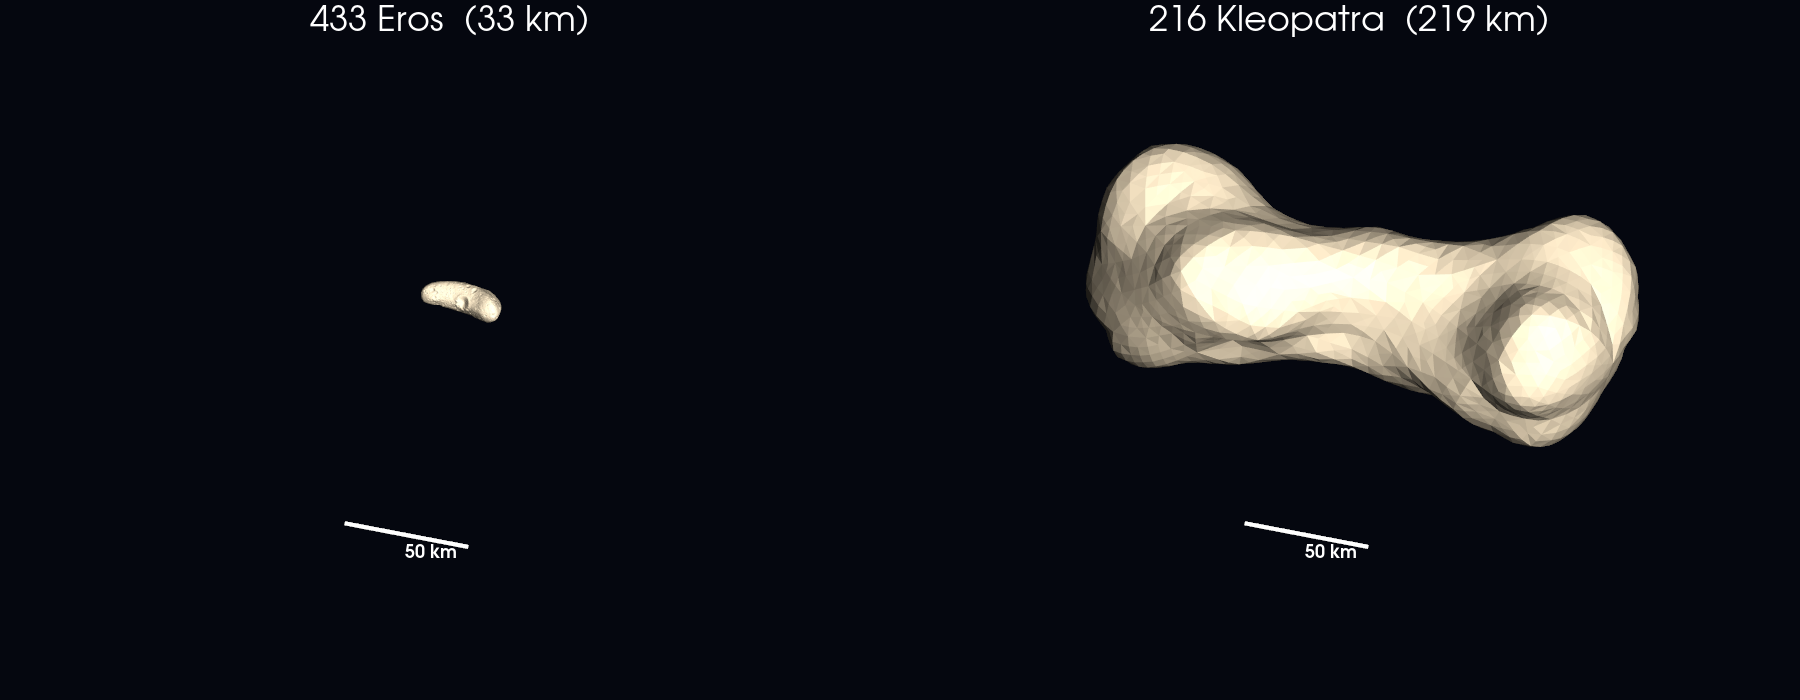
\includegraphics[width=0.85\textwidth]{Figures/bodies_same_scale.png}
\caption{The two test bodies drawn at the same scale: 433~Eros (Gaskell shape model, 33\,km
long) and the dog-bone shaped 216~Kleopatra (radar shape model, 219\,km long).}
\label{fig:bodies}
\end{figure}

\section{Type of problem}
A solution is a vector of numbers, so the problem is an \emph{arithmetic} problem
(Table~\ref{tab:ptype}). It is strictly \emph{mixed-integer}: the orbit variables and the
duration are real numbers, while one on/off switch per spacecraft slot is binary. It is not a
permutation problem, because exchanging two spacecraft gives the same fleet.

\begin{table}[htbp]
\centering
\caption{Classification of the optimisation problem}
\label{tab:ptype}
\footnotesize
\begin{tabularx}{\textwidth}{@{}p{2.0cm}p{3.6cm}X@{}}
\toprule
Type & A solution is \dots & Our problem? \\
\midrule
Permutation & an ordering of items & No: nothing is ordered; swapping two spacecraft gives the same fleet. \\
Binary & a string of 0/1 choices & Partly: the slot switches $s_i$ are 0/1, the orbits are not. \\
Arithmetic & a vector of real or integer numbers & Yes: $T$, $a_i$, $\iota_i$, $\Omega_i$, $M_{0,i}$ are real, $s_i$ is integer (mixed-integer). \\
\bottomrule
\end{tabularx}
\end{table}

Three properties make the problem hard for an optimiser and motivate a meta-heuristic:
\begin{itemize}
\item \textbf{Black box.} The fitness comes from a full mission simulation (orbits, rotation,
ray casting, sunlight, batteries); there is no formula to differentiate.
\item \textbf{Flat regions.} An orbit beyond the camera's usable range photographs nothing,
so many poor designs share almost the same fitness.
\item \textbf{Variable size.} The number of flying spacecraft is itself a decision, so part of
the vector is ignored whenever a slot is switched off.
\end{itemize}

\section{Decision variables}
The decision vector has one head variable, the mission duration $T$, followed by $N_{\max}$
\emph{slots} of five variables each (Table~\ref{tab:vars}):
\begin{equation}
\mathbf{x}=\bigl[\,T,\;\mathbf{y}_1,\;\dots,\;\mathbf{y}_{N_{\max}}\,\bigr],\qquad
\mathbf{y}_i=\bigl[a_i,\;\iota_i,\;\Omega_i,\;M_{0,i},\;s_i\bigr]\ \text{(slot $i$)},\qquad \dim\mathbf{x}=1+5N_{\max}
\label{eq:x}
\end{equation}
Slot $i$ flies a spacecraft when its switch $s_i=1$; the number of spacecraft is therefore
\begin{equation}
N=\sum_{i=1}^{N_{\max}}s_i,\qquad 1\le N\le N_{\max}.
\label{eq:N}
\end{equation}
The orbit numbers of a switched-off slot are carried along unused. A fixed-length vector lets
every algorithm (SA and GA now, PSO later) treat a design as one point in a box, while the
optimiser still decides the fleet size. With $N_{\max}=5$ the vector has 26 entries, with
$N_{\max}=10$ it has 51.

\begin{table}[htbp]
\centering
\caption{Decision variables. Every orbit is circular ($e=0$), so the argument of periapsis has
no meaning; the radius $a_i$ is the orbit's semi-major axis.}
\label{tab:vars}
\footnotesize
\begin{tabularx}{\textwidth}{@{}p{1.3cm}Xp{1.9cm}p{3.2cm}@{}}
\toprule
Symbol & Meaning & Type & Domain \\
\midrule
$T$ & mission duration & continuous & $[T_{\min},T_{\max}]$ (days) \\
$a_i$ & orbit radius of slot $i$ & continuous & $[r_{\min},r_{\max}]$ (km) \\
$\iota_i$ & inclination (tilt of the orbit to the asteroid equator) & continuous & $[0^\circ,180^\circ]$ \\
$\Omega_i$ & longitude of the ascending node (where the orbit crosses the equator) & continuous, periodic & $[0^\circ,360^\circ)$ \\
$M_{0,i}$ & mean anomaly at $t=0$ (where the spacecraft starts on its orbit) & continuous, periodic & $[0^\circ,360^\circ)$ \\
$s_i$ & slot switch: 1 = the slot flies a spacecraft, 0 = unused & binary & $\{0,1\}$ \\
\bottomrule
\end{tabularx}
\end{table}

Compared with Milestone~2, the eccentricity $e_i$, the argument of periapsis $\omega_i$ and
the scanner type $t_i$ were removed (circular orbits, one camera for all spacecraft), and
$T$ and the switches $s_i$ were added.

\section{Objectives}
Four quantities describe a design. Coverage and mission time lie in $[0,1]$; fleet cost and energy
use a fixed ten-spacecraft reference and may exceed one for fleets larger than that reference.

\textbf{Coverage $C$ (maximised).} Let $u_f=1$ if facet $f$ of area $A_f$ was photographed by
at least one spacecraft within the mission, under all the image-quality rules of
Section~\ref{sec:visibility}. Only facets that the Sun lights at some time can ever be
photographed, so coverage is measured against the sunlit area $A^{*}$:
\begin{equation}
C=\frac{S_a}{A^{*}},\qquad S_a=\sum_f A_f\,u_f,\qquad A^{*}=\sum_{f:\,\text{lit at some }t\le T_{\max}}A_f .
\label{eq:C}
\end{equation}

\textbf{Fleet cost $Z$ (minimised).} Each spacecraft costs a bus (1.0) plus its camera (0.2).
The total is divided by the cost of a reference fleet of $n_{\mathrm{ref}}=10$ spacecraft, so
\begin{equation}
Z=\frac{N\,(c_{\mathrm{bus}}+c_{\mathrm{cam}})}{n_{\mathrm{ref}}\,(c_{\mathrm{bus}}+c_{\mathrm{cam}})}=\frac{N}{10}.
\label{eq:Z}
\end{equation}
A fixed reference (instead of $N_{\max}$) makes one spacecraft cost the same in every case
study, so cases with different $N_{\max}$ are comparable and oversized fleets remain penalised.

\textbf{Energy $E$ (minimised).} Half propellant, half electricity:
\begin{align}
E&=\tfrac12\,\frac{\sum_i\Delta V_i}{n_{\mathrm{ref}}\,3v_0}
 +\tfrac12\,\frac{\sum_i E_{\mathrm{elec},i}}{n_{\mathrm{ref}}\,E_{\mathrm{ref}}},\label{eq:E}\\
E_{\mathrm{elec},i}&=P_{\mathrm{base}}\,T+n_{\mathrm{img},i}\,(e_{\mathrm{img}}+e_{\mathrm{tx}}),\qquad
E_{\mathrm{ref}}=(P_{\mathrm{base}}+P_{\mathrm{cam}}+P_{\mathrm{tx}})\,T_{\max}\nonumber
\end{align}
$\Delta V_i$ is the velocity change needed to reach the orbit from a common circular,
equatorial arrival orbit of radius $r_0$ (Section~\ref{sec:dv}); $3v_0$, with
$v_0=\sqrt{\mu/r_0}$, is larger than any such manoeuvre. $n_{\mathrm{img},i}$ is the number of
frames spacecraft $i$ takes, each costing the exposure energy $e_{\mathrm{img}}$ and the
energy $e_{\mathrm{tx}}$ to send it to Earth.

\textbf{Mission time (minimised).} The duration enters as $T/T_{\max}$.

\section{Fitness function}
The four objectives are combined into one weighted fitness that both \ac{SA} and \ac{GA} minimise:
\begin{equation}
\boxed{\;J(\mathbf{x})=w_C\,(1-C)+w_Z\,Z+w_E\,E+w_T\,\frac{T}{T_{\max}}\;}
\label{eq:J}
\end{equation}
with the weights $(w_C,w_Z,w_E,w_T)=(0.5,\,0.15,\,0.15,\,0.2)$.
Coverage is the only maximised quantity; it enters as $1-C$, the share of the sunlit area that
was missed, so maximising $C$ and minimising $1-C$ have the same optimum. The weights add to one.
For fleets no larger than the reference, the terms are in the usual unit range; for
$N>n_{\mathrm{ref}}$, the fixed-reference cost and energy terms can exceed one by design. The ideal
limiting interpretation $J=0$ would be the whole sunlit area imaged instantly at no cost and no
energy. The form $1-C$ is used rather than $1/C$ because $1/C$ is
infinite for a fleet that images nothing (common among random designs) and would make the last,
hardest percentages of coverage almost worthless. With these weights one more spacecraft
($w_Z\Delta Z=0.015$, plus its share of the energy term) pays for itself only if it adds about
three to four percentage points of coverage, and
shortening the mission by 10\,\% of $T_{\max}$ is worth four points; this is what stops the
optimiser from simply sending every spacecraft for as long as possible.

\section{Constraints}
\label{sec:constraints}
Every constraint is written as $g\le0$ and normalised, so a positive value is the relative size
of the violation (Table~\ref{tab:constraints}).

\begin{table}[htbp]
\centering
\caption{Constraints. Index $i$ runs over the flying spacecraft ($s_i=1$), $t_k=k\,\Delta t$ over
the time steps of the mission.}
\label{tab:constraints}
\footnotesize
\begin{tabularx}{\textwidth}{@{}p{2.2cm}Xp{4.6cm}p{1.6cm}@{}}
\toprule
Name & Meaning & Normalised form ($\le0$ when satisfied) & Checked \\
\midrule
fleet size & at least one spacecraft, switches binary & $N\ge1$, $s_i\in\{0,1\}$ & before engine \\
duration & mission length within its range & $\max(T_{\min}-T,\,T-T_{\max})/T_{\max}$ & before engine \\
$g_1$ minimum radius & no orbit inside the safety sphere $r_{\min}=\kappa R_{\max}$ & $\max_i (r_{\min}-a_i)/r_{\min}$ & before engine \\
$g_2$ maximum radius & two-body model stays valid, camera stays useful & $\max_i (a_i-r_{\max})/r_{\max}$ & before engine \\
inclination & physical range of $\iota$ & $\max_i\max(-\iota_i,\,\iota_i-180^\circ)/180^\circ$ & before engine \\
$g_3$ separation & no two spacecraft closer than $d_{\mathrm{sep}}$ at any step $t_k\le T$ & $\bigl(d_{\mathrm{sep}}-\min_{i<j,\,k}\|\mathbf{r}_i(t_k)-\mathbf{r}_j(t_k)\|\bigr)/d_{\mathrm{sep}}$ & before engine \\
$g_4$ battery & state of charge never below $q_{\min}=20\,\%$ at any step $t_k\le T$ & $(q_{\min}-\min_{i,k}q_i(t_k))/q_{\min}$ & after engine \\
\bottomrule
\end{tabularx}
\end{table}

For a circular orbit the periapsis and apoapsis both equal $a_i$, so $g_1$ and $g_2$ reduce to
bounds on $a_i$. $\Omega_i$ and $M_{0,i}$ are angles: every real value is a valid orbit, so they
need no constraint. All constraints except the battery are checked \emph{before} the expensive
simulation; a design that fails them is never simulated (Chapter~\ref{ch:sa}). Infeasible designs
receive a penalised cost above every feasible $J$, so the optimiser can still rank them by how
badly they fail:
\begin{equation}
J_{\mathrm{inf}}(\mathbf{x})=J_0+\rho\sum_j\bigl[\max(0,g_j(\mathbf{x}))\bigr]^2,\qquad J_0=\rho=10^3 .
\label{eq:penalty}
\end{equation}

\section{Parameters}
The method is independent of the body: Table~\ref{tab:params} lists the values for both bodies.
All Kleopatra distances keep the same proportions to the body as for Eros
($r_{\min}=1.5R_{\max}$, $r_{\max}\approx3.8\,r_{\min}$), which needs a coarser resolution limit
of 20\,m per pixel (as Dawn mapped the similar-sized Vesta~\cite{raymond2011}); Kleopatra's mass is
that of Bro\v{z} et al.~\cite{broz2021}. Everything else is identical.

\begin{table}[htbp]
\centering
\caption{Mission and problem parameters}
\label{tab:params}
\footnotesize
\begin{tabularx}{\textwidth}{@{}Xp{1.6cm}p{3.3cm}p{3.3cm}@{}}
\toprule
Parameter & Symbol & 433 Eros & 216 Kleopatra \\
\midrule
Gravitational parameter & $\mu$ & $4.463\times10^{-4}$\,km$^3$/s$^2$ & $0.1982$\,km$^3$/s$^2$ \\
Rotation period & $P_{\mathrm{rot}}$ & 5.27\,h & 5.385\,h \\
Shape model used in the search & --- & Gaskell, 1\,499 facets\textsuperscript{a} & radar, 4\,092 facets \\
Farthest surface point & $R_{\max}$ & 17.6\,km & 114.2\,km \\
Surface area & --- & 1\,124\,km$^2$ & 52\,186\,km$^2$ \\
Orbit radius range & $r_{\min}$, $r_{\max}$ & 26.5 -- 100\,km & 171.2 -- 650\,km \\
Minimum separation & $d_{\mathrm{sep}}$ & 2\,km & 10\,km \\
Resolution limit & $\mathrm{GSD}_{\max}$ & 3\,m & 20\,m \\
Usable camera range & $\ell_{\max}$ & 58.6\,km & 390.8\,km \\
Arrival orbit radius & $r_0$ & 50\,km & 320\,km \\
\midrule
Camera (all spacecraft) & $\psi,\,p$ & \multicolumn{2}{p{6.6cm}}{$6^\circ$ field of view, $2048\times2048$ pixels} \\
Maximum emission angle & $\eta_{\max}$ & \multicolumn{2}{p{6.6cm}}{$65^\circ$} \\
Lighting & --- & \multicolumn{2}{p{6.6cm}}{Sun $\ge20^\circ$ above the facet horizon and no cast shadow} \\
Time step & $\Delta t$ & \multicolumn{2}{p{6.6cm}}{10\,min (one frame per step, set by the 503\,s downlink of a frame)} \\
Power & --- & \multicolumn{2}{p{6.6cm}}{$P_{\mathrm{base}}=50$\,W, $P_{\mathrm{cam}}=10$\,W, $P_{\mathrm{tx}}=30$\,W, solar 180\,W, battery 200\,Wh} \\
Energy per frame & $e_{\mathrm{img}},e_{\mathrm{tx}}$ & \multicolumn{2}{p{6.6cm}}{100\,J, 15.1\,kJ} \\
Minimum battery charge & $q_{\min}$ & \multicolumn{2}{p{6.6cm}}{20\,\%} \\
Weights & $w_C,\dots,w_T$ & \multicolumn{2}{p{6.6cm}}{0.5, 0.15, 0.15, 0.2} \\
Cost reference & $n_{\mathrm{ref}}$ & \multicolumn{2}{p{6.6cm}}{10 spacecraft} \\
Penalty & $J_0,\rho$ & \multicolumn{2}{p{6.6cm}}{$10^3$, $10^3$} \\
\bottomrule
\end{tabularx}
\par\smallskip
\parbox{\textwidth}{\scriptsize \textsuperscript{a}\,The matched GA--SA comparison of
Section~\ref{sec:garesults} uses a 3\,000-facet copy; every final Eros design is re-checked on a
6\,000-facet copy (validation V7).}
\end{table}

\section{Assumptions}
\begin{itemize}
\item \textbf{Two-body dynamics.} Each spacecraft follows an ideal circular Kepler orbit around
the asteroid's centre of mass; the irregular gravity field, solar radiation pressure and
third bodies are ignored.
\item \textbf{Uniform rotation} of the asteroid about its inertial $z$ axis.
\item \textbf{Fixed Sun direction} in inertial space during the mission (sub-solar latitude
$0^\circ$, equinox).
\item \textbf{Nadir pointing.} Every camera points at the asteroid's centre; one frame is taken
per time step whenever at least one facet is visible.
\item \textbf{Discrete time.} Visibility, separation and battery are checked at the time steps
$t_k$ only.
\item \textbf{Facet-level observation.} A facet counts as photographed if its centre passes all
the tests of Section~\ref{sec:visibility}.
\end{itemize}
